\documentclass[tikz,border=4pt]{standalone}

% Pure TikZ — no pgfplots / fontspec / siunitx so the document builds
% on a minimal TinyTeX install (see figgen tikz_backend).
\usetikzlibrary{arrows.meta, positioning, calc, patterns,
                decorations.pathmorphing}

% -- B&W-safe palette (near-black ink + mid-grey fill) ----------------
\definecolor{steel}{HTML}{1a1a1a}
\definecolor{greyFill}{HTML}{c8c8c8}
\definecolor{sandFill}{HTML}{ece6d4}
\definecolor{scourFill}{HTML}{f5efe1}
\definecolor{accent}{HTML}{2a2a2a}
\definecolor{forceMoved}{HTML}{cc3333}

% Common dimensions
\def\bucketW{1.2}
\def\bucketH{1.4}
\def\bucketSpacing{2.0}
\def\towerH{5.6}
\def\nacelleW{1.7}
\def\nacelleH{0.55}
\def\mudlineY{0}
\def\scourDepth{0.55}

% ====================================================================
\begin{document}
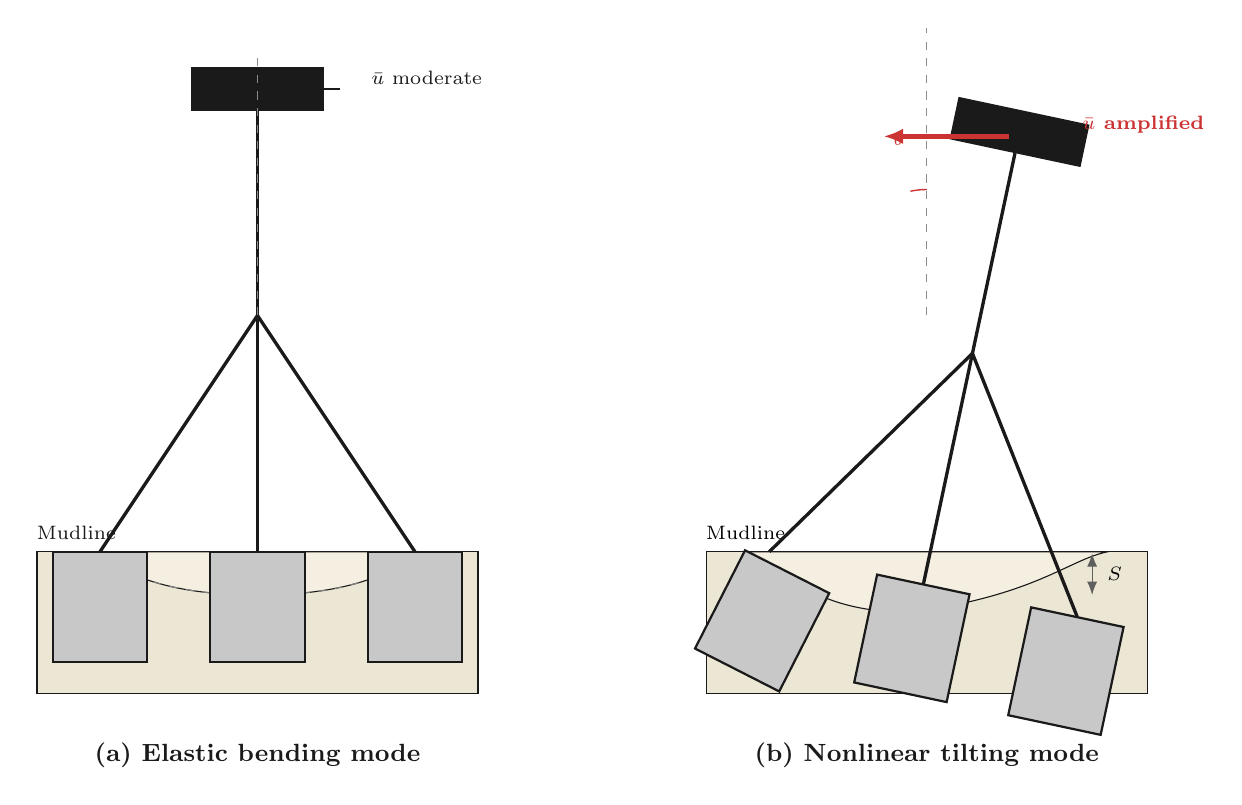
\begin{tikzpicture}[
    font=\sffamily\small,
    scale=1.0,
    every node/.style={font=\sffamily\footnotesize},
    bucket/.style={draw=steel, line width=0.8pt, fill=greyFill},
    frame/.style={draw=steel, line width=1.2pt},
    soil/.style={draw=steel, line width=0.4pt, fill=sandFill},
    scour/.style={draw=steel, line width=0.4pt, fill=scourFill,
                  pattern color=steel!40},
    force/.style={-{Latex[length=2.5mm,width=2mm]}, line width=1.0pt},
    dim/.style={Latex-Latex, line width=0.4pt, draw=steel!70},
    ]

% ====================================================================
% Panel (a) — Elastic bending mode
% ====================================================================
\begin{scope}[local bounding box=panelA]

\def\ox{0}
\def\oy{0}

% Soil (sand) block
\fill[soil] (\ox-2.8,\oy-1.8) rectangle (\ox+2.8,\oy);
\draw[frame, line width=0.5pt] (\ox-2.8,\oy) -- (\ox+2.8,\oy)
  node[midway, above=1pt, xshift=-2.3cm, font=\scriptsize, color=steel]{Mudline};

% Scour hole around the buckets (shallow symmetric)
\fill[scour] (\ox-2.3,\oy) .. controls (\ox-1.8,\oy-0.1) and (\ox-1.5,\oy-\scourDepth)
  .. (\ox,\oy-\scourDepth)
  .. controls (\ox+1.5,\oy-\scourDepth) and (\ox+1.8,\oy-0.1)
  .. (\ox+2.3,\oy) -- cycle;
\draw[dashed, line width=0.4pt, color=steel!55]
  (\ox-2.3,\oy) .. controls (\ox-1.8,\oy-0.1) and (\ox-1.5,\oy-\scourDepth)
  .. (\ox,\oy-\scourDepth)
  .. controls (\ox+1.5,\oy-\scourDepth) and (\ox+1.8,\oy-0.1)
  .. (\ox+2.3,\oy);
\draw[dim] (\ox+2.1,\oy-0.02) -- (\ox+2.1,\oy-\scourDepth)
  node[midway, right=2pt, font=\scriptsize]{$S$};

% Three buckets (left, center, right) sitting vertical
\foreach \d in {-\bucketSpacing, 0, \bucketSpacing}{
    \fill[greyFill, draw=steel, line width=0.8pt]
      (\ox+\d-\bucketW/2,\oy-\bucketH)
      rectangle (\ox+\d+\bucketW/2,\oy);
}

% Tripod frame (three struts converging at tower base)
\def\legTop{3.0}
\draw[frame] (\ox-\bucketSpacing,\oy) -- (\ox,\oy+\legTop);
\draw[frame] (\ox,\oy)                -- (\ox,\oy+\legTop);
\draw[frame] (\ox+\bucketSpacing,\oy) -- (\ox,\oy+\legTop);

% Tower and nacelle (straight, vertical — elastic bending is a tiny
% deformation so at a schematic scale the tower is drawn plumb)
\draw[frame] (\ox,\oy+\legTop) -- (\ox,\oy+\towerH);
\fill[steel] (\ox-\nacelleW/2,\oy+\towerH)
  rectangle (\ox+\nacelleW/2,\oy+\towerH+\nacelleH);

% Reference (plumb) dashed vertical line
\draw[dashed, line width=0.3pt, steel!50]
  (\ox,\oy+\legTop) -- (\ox,\oy+\towerH+\nacelleH+0.2);

% Displacement arrow at nacelle — small moderate "u-bar"
\draw[force, color=steel]
  (\ox+\nacelleW/2+0.2,\oy+\towerH+\nacelleH/2)
  -- +(-0.8,0);
\node[font=\scriptsize, color=steel]
  at (\ox+\nacelleW/2+1.3,\oy+\towerH+\nacelleH/2+0.15)
  {$\bar{u}$ moderate};

% Panel title
\node[font=\bfseries\small, color=steel, anchor=north]
  at (\ox,\oy-2.3) {(a) Elastic bending mode};

\end{scope}

% ====================================================================
% Panel (b) — Nonlinear tilting mode (right of panel A)
% ====================================================================
\begin{scope}[local bounding box=panelB, shift={(8.5,0)}]

\def\ox{0}
\def\oy{0}

% Soil
\fill[soil] (\ox-2.8,\oy-1.8) rectangle (\ox+2.8,\oy);
\draw[frame, line width=0.5pt] (\ox-2.8,\oy) -- (\ox+2.8,\oy)
  node[midway, above=1pt, xshift=-2.3cm, font=\scriptsize]{Mudline};

% Scour (asymmetric — deeper on the upwind side)
\fill[scour] (\ox-2.3,\oy) .. controls (\ox-1.8,\oy-0.2) and (\ox-1.5,\oy-\scourDepth*1.4)
  .. (\ox-0.2,\oy-\scourDepth*1.4)
  .. controls (\ox+1.4,\oy-\scourDepth*1.0) and (\ox+1.8,\oy-0.1)
  .. (\ox+2.3,\oy) -- cycle;
\draw[dim] (\ox+2.1,\oy-0.02) -- (\ox+2.1,\oy-\scourDepth)
  node[midway, right=2pt, font=\scriptsize]{$S$};

% Buckets: upwind (leftmost) has yielded and rotated; others tilt with
% the whole foundation about the yielded bucket.
\def\tiltDeg{12}
\foreach \d [count=\i from 1] in {-\bucketSpacing, 0, \bucketSpacing}{
    \ifnum\i=1
      % Tilted + sunk upwind bucket (left-most)
      \begin{scope}[rotate around={-\tiltDeg-15:(\ox+\d,\oy-\bucketH/2)},
                    shift={(\ox+\d,\oy-0.2)}]
        \fill[greyFill, draw=steel, line width=0.8pt]
          (-\bucketW/2,-\bucketH) rectangle (\bucketW/2,0);
      \end{scope}
    \else
      % Other buckets rotate about the yielded bucket — draw tilted
      \begin{scope}[rotate around={-\tiltDeg:(\ox-\bucketSpacing,\oy)}]
        \fill[greyFill, draw=steel, line width=0.8pt]
          (\ox+\d-\bucketW/2,\oy-\bucketH)
          rectangle (\ox+\d+\bucketW/2,\oy);
      \end{scope}
    \fi
}

% Tilted tripod frame and tower (whole assembly rotated about leftmost bucket)
\def\legTop{3.0}
\begin{scope}[rotate around={-\tiltDeg:(\ox-\bucketSpacing,\oy)}]
  \draw[frame] (\ox-\bucketSpacing,\oy) -- (\ox,\oy+\legTop);
  \draw[frame] (\ox,\oy)                -- (\ox,\oy+\legTop);
  \draw[frame] (\ox+\bucketSpacing,\oy) -- (\ox,\oy+\legTop);
  \draw[frame] (\ox,\oy+\legTop) -- (\ox,\oy+\towerH);
  \fill[steel] (\ox-\nacelleW/2,\oy+\towerH)
    rectangle (\ox+\nacelleW/2,\oy+\towerH+\nacelleH);
\end{scope}

% Reference plumb line (from tower base upward)
\draw[dashed, line width=0.3pt, steel!50]
  (\ox,\oy+\legTop) -- (\ox,\oy+\towerH+\nacelleH+0.5);

% Tilt angle arc + theta label
\draw[line width=0.5pt, color=forceMoved]
  (\ox,\oy+\towerH-1.0) arc (90:90+\tiltDeg:1.0);
\node[font=\scriptsize, color=forceMoved]
  at (\ox-0.35,\oy+\towerH-0.35) {$\theta$};

% Displacement arrow at nacelle — larger + bold (amplified u-bar)
\draw[force, color=forceMoved, line width=1.6pt]
  (\ox+\nacelleW/2+0.2,\oy+\towerH+\nacelleH/2-0.6)
  -- +(-1.6,0);
\node[font=\scriptsize\bfseries, color=forceMoved]
  at (\ox+\nacelleW/2+1.9,\oy+\towerH+\nacelleH/2-0.45)
  {$\bar{u}$ amplified};

% Panel title
\node[font=\bfseries\small, color=steel, anchor=north]
  at (\ox,\oy-2.3) {(b) Nonlinear tilting mode};

\end{scope}

\end{tikzpicture}
\end{document}
